\section{Perspectiva geométrica}
\subsection{Teoría para la perspectiva geométrica}

Antes de empezar con el contexto de la perspectiva geométrica, es imprescindible dar una introducción a la teoría necesaria para entender el funcionamiento del método de mínimos cuadrados:

\subsubsection{Teorema descomposición ortogonal}

Sea $W$ un subespacio de $\R^n$ y $x$ un vector en $\R^n$. Entonces se puede escribir de forma única a $x$ como la suma de $x_w $ y $x_w^\perp$, donde el primero, $x_w $, es un vector perteneciente a $W$ y $x_w^\perp$ es un vector perteneciente a $W_\perp = \{ x \in \R^n |\ x\cdot y = 0 \; \forall \; y \in W\}$, llamado subespacio ortogonal a W. \\

\mathbf{Demostración}: Sea $m = dim(W)$ y $n - m = dim(W_\perp)$. Al ser ambos subespacios de $\R^n$, cuentan con base. Denotemos entonces los conjuntos, $B_W = \{v_{w, \\ 1},{v_{w, \\ 2}, \dots, {v_{w, \\ m}  \}$ y $B_{W'} = \{v_{w', \\ 1},{v_{w', \\ 2}, \dots, {v_{w', \\ n-m} \}$, cada uno siendo la base de los subespacios $W$ y $W_\perp$, respectivamente.

Notemos ahora que, al ser ortogonales entre ellos, la unión de ambas bases generará una base para $\R^n$, debido a que si existiesen coeficientes $C = \{c_1, c_2, \dots, c_n \}$, donde alguno de ellos es distinto de 0,  tal que 
$$ \sum_{i = 1}^{m}v_{w, \\ i}*c_i \; + \sum_{i = 1}^{n-m}v_{w', \\ i}*c_{i\\ + m} = 0$$

Entonces se tendria que:

$$ \sum_{i = 1}^{m}v_{w, \\ i}*c_i \; \cdot \sum_{i = 1}^{n-m}v_{w', \\ i}*c_{i\\ + m} =  - \sum_{i = 1}^{n-m}v_{w', \\ i}*c_{i\\ + m}\;\cdot \sum_{i = 1}^{n-m}v_{w', \\ i}*c_{i\\ + m}$$

La contradicción estaría en que el lado izquierdo tendría un valor de 0 ya que son vectores ortogonales, mientras que el lado derecho solo tendría un valor de 0 cuando los coeficientes $c_{i\\ + m}$ son 0. Si estos fuesen 0, entonces: 

$$ \sum_{i = 1}^{n}v_{w, \\ i}*c_{i} =  0$$

Que, como es una combinación de elementos de la base $B_W$ y esta es linealmente independiente, implica que los coeficientes $c_i$ tienen un valor de 0. 

De aquí se tiene entonces que todos los coeficientes del conjunto $C$ son 0, de lo que se concluye que la unión de las dos bases de los subespacios respectivos generaría una base para $\R^n$.

Habiendo demostrado entonces que $B = B_W \,\cup \, B_{W'}$ es una base para $\R^n$, el vector $x$ se puede representar como combinación lineal de esta, que se podría particionar de la siguiente forma:
$$ x = \sum_{i = 1}^{m}v_{w, \\ i}*c_i \; + \sum_{i = 1}^{n-m}v_{w', \\ i}*c_{i\\ + m}
$$

Como se había denotado en la demostración anterior, la primera sumatoria correspondería con un vector en $W$ y la segunda sumatoria correspondería con un vector en $W_\perp$.

Ahora, la unicidad de esta representación viene por la misma independencia lineal de la base $B$.

\textbf{Teorema 3.1.2} \\
Teniendo el resultado anterior y denotando que, para el caso del problema de mímimos cuadrados, el subespacio $W$ corresponde al subespacio $col(A)$ de la ecuación $Ax = b$, donde $A $ es una matriz $m*n$, $x$ es un vector en $\R^n$ y $b$ es un vector en $\R^m$, se propone que la siguiente ecuación matricial tiene una solución $c$ en $R^n$ dado un vector de $y$ definido en $\R^m$:

$$A^TAc = A^Ty$$

Donde $Ac$ corresponde al vector $y_w$. \\

\mathbf{Demostración}: Usando el teorema anterior, se sabe que $y = y_w \; + y_{w}^\perp$, de forma que $y_w^\perp =\, y \;- y_w$. Ahora, es importante notar que, como $y_w^\perp \in W_\perp$, entonces $y_w^\perp \in Nul(A^T)$. Esto se puede notar facilmente debido a que, como $y_w^\perp$ es ortogonal a las columnas de $A$, entonces $A^Ty_w^\perp$ tiene en la entrada $i$ el producto punto entre $y_w^\perp$ y el vector columna $i$ de $A$, que será 0 para cualquier $i$. 

De esta forma, se tiene que, multiplicando por $A^T$ en ambos lados: 
$$ A^Ty_w^\perp =\, A^T(y \;- y_w)
$$

Que da que:

$$ 0 = A^T(y - y_w)  \rightarrow A^Ty = A^Ty_w
$$

Como $y_w = Ac$ para algún $c \in \R^n$, podemos reemplazar y se obtiene que:

$$A^TAc = A^Ty$$

Y se llega al resultado requerido.

\subsection{Definición de una solución de mínimos cuadrados}

Ya teniendo claro las bases teóricas, definamos qué es una solución de mínimos cuadrados. 

\\ Sea $A$ una matriz $m*n$ y sea $b$ un vector en $R^m$. Una solución de mínimos cuadrados de la ecuación $Ax = b$ es un vector $\hat{x}$ tal que:
$$ dist (b, A\hat{x}) \le dist(b, Ax) \;\;\;\;\;\;\; \forall x \in \R^n
$$

Es decir, es el vector en $col(A)$ más cercano a $b$. Se puede ver de la siguiente forma:

\begin{wrapfigure}
    \centering
    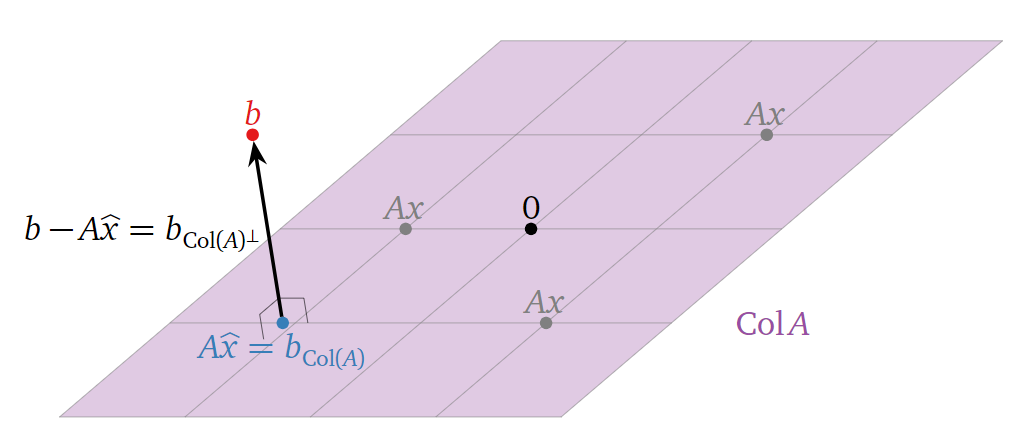
\includegraphics[width=1\linewidth]{image_2025-01-17_190701322.png}
    \caption{Obtenido de (The Method of Least Squares, n.d.)}
\end{wrapfigure}

\\

En la gráfica se aprecia la relación de ortogonalidad entre $b_{col(A)}$ y $b_{col(A)^\perp}$, que corresponden con la descomposición ortogonal de $b$ con respecto a $col(A)$. Esta es justo la cualidad que permite que $A\hat{x}$ sea el vector en $col(A)$ más cercano a $b$.
 
\\ Ahora, teniendo en cuenta lo demostrado, se tiene que $\hat{x}$ es la solución de la siguiente ecuación matricial:

$$ A^TA\hat{x} = A^Tb$$

Esto da una idea general de como solucionar un problema de mínimos cuadrados. A continuación se muestra un ejemplo:

\\ Con: $$A = \begin{bmatrix}
0 & 1 \\
1 & 1 \\
2 & 1
\end{bmatrix} \;\;\text{y} \;\; b = \begin{bmatrix} 6 \\ 0\\ 0 \end{bmatrix}$$

Halle la solución para el problema de mínimos cuadrados.

\\Solución: 

Primero, hallemos $A^T$, que corresponde a la matriz transpuesta:

$$A^T = \begin{bmatrix}
0 & 1 & 2\\
1 & 1 & 1 \\
\end{bmatrix}$$

Con esta, podrémos calcular el producto de matrices $A^TA$:

$$A^TA = \begin{bmatrix}
0 & 1 & 2\\
1 & 1 & 1
\end{bmatrix} \begin{bmatrix}
0 & 1 \\
1 & 1 \\
1 & 2
\end{bmatrix}  = \begin{bmatrix}
5 & 3 \\
3 & 3 \\
\end{bmatrix}$$

Por otro lado, $A^Tb$ también se calcula:

$$A^Tb = \begin{bmatrix}
0 & 1 & 2\\
1 & 1 & 1
\end{bmatrix}\begin{bmatrix} 6 \\ 0\\ 0 \end{bmatrix} =\begin{bmatrix} 0 \\ 6\\  \end{bmatrix} $$

De esta forma, se llega al siguiente sistema lineal de ecuaciones:

$$ \begin{bmatrix}
5 & 3 \\
3 & 3 \\
\end{bmatrix}\begin{bmatrix} \hat{x_1} \\ \hat{x_2}\\ \end{bmatrix} =\begin{bmatrix} 0 \\ 6\\  \end{bmatrix} $$

Cuya solución es: 
$$
\begin{bmatrix} \hat{x_1} \\ \hat{x_2}\\ \end{bmatrix} =\begin{bmatrix} -3 \\ 5\\  \end{bmatrix} $$
La visualización de la solución se puede ver a continuación:

\begin{wrapfigure}
    \centering
    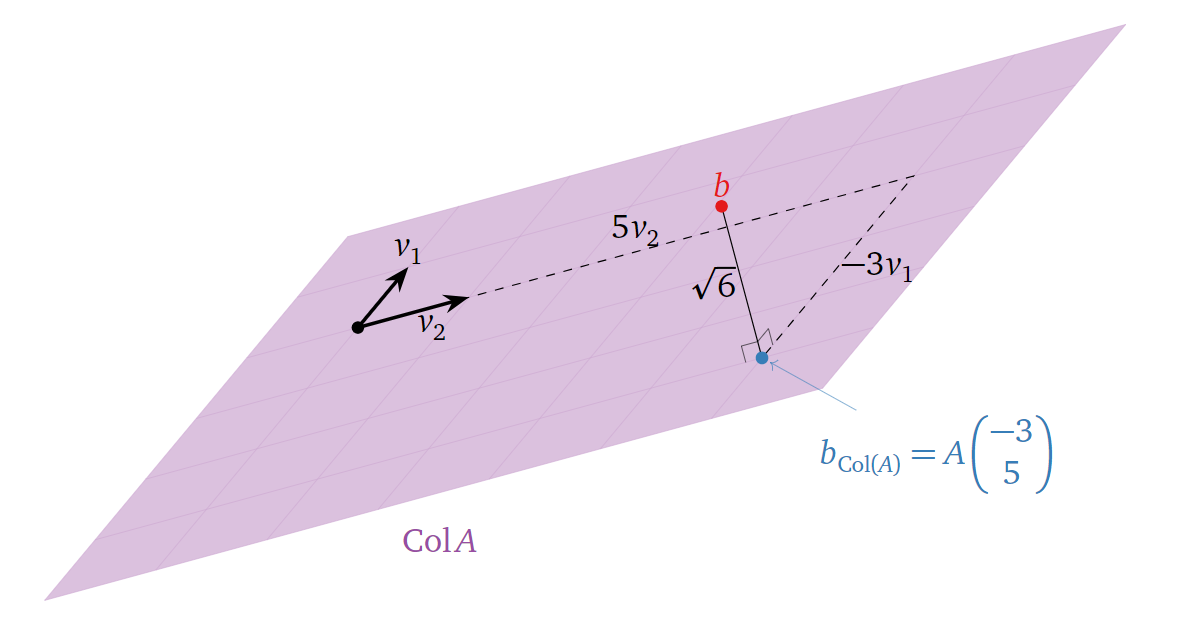
\includegraphics[width=1\linewidth]{image_2025-01-17_194708435.png}
    \caption{Obtenido de (The Method of Least Squares, n.d.)}
\end{wrapfigure}

En este caso, la distancia entre $b$ y $\hat{x}$ es de $\sqrt{6}$.

